\chapter{Marco teórico}
\label{ch:teoria}

En el presente capítulo se repasan los conceptos que fundamentan el proceso de diseño de un controlador de una planta de laboratorio como el péndulo amortiguado a hélice, mediante prácticas de aprendizaje reforzado.

\section{Péndulo amortiguado de motor con hélice}

El péndulo amortiguado de motor con hélice (PAMH) se trata de un sistema extrapolado de un péndulo simple, compuesto de un motor con hélice, controlado por una señal de modulación por ancho de pulsos (\textit{pulse-width modulation}, PWM), una masa pequeña colocada en contrapeso al motor, el péndulo resultante de los brazos de aluminio y pesos correspondientes, así como soportes de aluminio de baja fricción, componentes responsables de mantener la estructura. Un modelo simplificado del sistema se muestra en la figura \ref{fig:modpen} junto con las magnitudes y vectores utilizados en la generación de modelo analítico del sistema \cite{PAMH1}.

\begin{figure}[h]
	\centering
	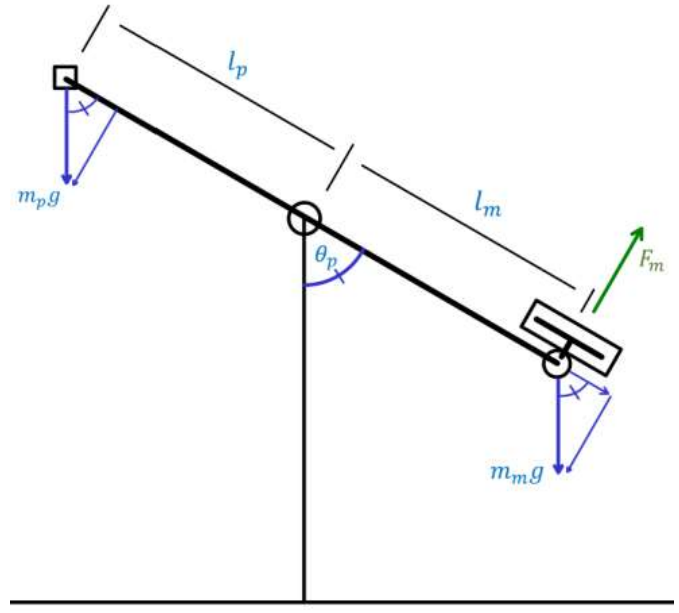
\includegraphics[scale=0.3]{fig/new/ModeloPendulo.png}
	\caption{Modelo simplificado del PAMH. Fuente: \cite{PAMHppt}}
	\label{fig:modpen}
\end{figure}

El objetivo principal  de dicho sistema es controlar la magnitud del ángulo $\theta_p$ medido entre la estructura y el péndulo, únicamente aplicando la señal PWM al motor que se encuentra a una distancia $l_m$ de la estructura y ejerce una fuerza $F_m$, que provoca el movimiento de su masa $m_m$ mientras, a una distancia de $l_p$ del centro, se encuentra una masa $m_p$ que contrarresta el movimiento.

\subsection{Modelo analítico del PAMH}

El modelado de sistemas físicos permite la elaboración de planes de trabajo con una base en común y bien sustentada en las características del entorno utilizado, permitiendo el diseño de controladores funcionales y eficientes. Este enfoque facilita la predicción del comportamiento del sistema bajo diversas condiciones operativas y la implementación de estrategias de control robustas, de manera que es común la elaboración de diagramas, como el caso de la figura \ref{fig:modpen} para la interpretación matemática \cite{Nise}.

El problema del péndulo suele ser abordado como un problema de leyes de Newton, donde se parte de la \textit{ley de movimiento rotacional de Newton} aplicada al modelo simplificado de la figura \ref{fig:modpen}.
\begin{equation}
\sum \tau = J_p\, \vec{a}
\label{ecu:sumatorques}
\end{equation}
La sumatoria de torques $\tau$ corresponde a la inercia del cuerpo péndulo $J_p$ por su aceleración ángular $\vec{a}$ \cite{Ogata}, de manera que la ecuación (\ref{ecu:sumatorques}) equivale a:
\[\tau_m - \tau_{mg} - \tau_{\beta} + \tau_{pg} = J_p \vec{a}\]
\begin{equation}
l_m\, F_m - l_m\, m_m g \,\sen(\theta_p)- l_m \,\beta \,\dot{\theta_p} + l_p\, m_p g\, \sen(\theta_p) = J_p\, \ddot{\theta_p}
\end{equation}
en donde $\beta$ corresponde a la constante de rozamiento en el eje central de la planta, constante comúnmente despreciable. Además, para deflexiones pequeñas se linealiza la ecuación con la aproximación $\sen(\theta_p) \approx \theta_p$. Las ecuaciones de estado son:
\[x_1 = \theta_p \qquad x_2 = \dot{\theta}_p \qquad y = x_1 = \theta_p\]
\begin{equation}
	\left \{ \begin{array}{lcc} \dot{x}_1 = x_2 \\ \\ \dot{x}_2 = -\dfrac{l_m \beta}{J_p} x_2 + (m_p l_p -m_m l_m)\dfrac{g}{J_p}x_1 +\dfrac{l_m}{J_p}F_m \end{array} \right.
	\label{ecu:sistemaPAMH}
\end{equation}
y la función de transferencia al aplicar el análisis en frecuencia:
\begin{equation}
T(s) = \frac{\theta_p(s)}{F_m(s)} = \frac{\dfrac{l_m}{J_p}}{s^2 + \dfrac{l_m\beta}{J_p}s +\dfrac{(l_m m_m-l_p m_p)g}{J_p}}
\end{equation}
punto desde el que se puede empezar a plantear alguna estrategia de control clásico al sistema o entorno, pero limitando al rango angular propiciado por la aproximación del componente trigonométrico.

Una consideración del procedimiento analítico realizado es que solo aproxima a la planta real, pues el modelo de la ecuación (\ref{ecu:sistemaPAMH}) no considera el movimiento mecánico producto de la holgura en el eje, o factores de resistencia mecánica por los cables eléctricos que toman la señal angular o llevan la energía al motor, o alteraciones con histéresis producto del movimiento de esos cables, factores que, acumulados, acarrean retos adicionales en el diseño de un controlador.

\section{Redes neuronales artificiales (RNA)}

Las RNA nacen de la experimentación para emular computacionalmente la capacidad del cerebro humano. El modelo usual de una neurona artificial se muestra en la figura \ref{fig:neurona} \cite{RNACaravaca}. Los valores de entrada $x_i$ se escalan por los pesos correspondientes $w_{ni}$, para luego sumarlos y transformarlos con la función de activación $\varphi(\cdot)$ (o también $f(\cdot)$), resultando en la salida \cite{RNACaravaca}:

\begin{equation}
y_i = \varphi \left(\sum^m_{j=1} w_{ij} x_j \right)
\label{ecu:neurona}
\end{equation}

\begin{figure}[h]
	\centering
	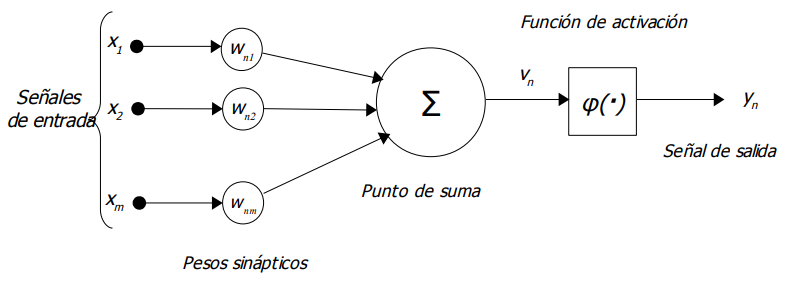
\includegraphics[scale=0.55]{fig/new/NeuronaRNA.png}
	\caption{Modelo de neurona artificial. Fuente: \cite{RNACaravaca}.}
	\label{fig:neurona}
\end{figure}

Un número $N$ de neuronas se interconecta dentro del sistema completo de la red neuronal artificial como se muestra en la figura \ref{fig:RNA}. Esta red recibe los vectores de entrada $\mathbf{x}$ y produce los vectores de salida $\mathbf{y}$. En el proceso, las capas ocultas producen los vectores $\mathbf{x}^{(n)}$ utilizando las matrices de pesos $\mathbf{A}_i$ que guardan los pesos correspondientes a cada neurona \cite{RNACaravaca} \cite{DataScience}.

\begin{figure}[h]
	\centering
	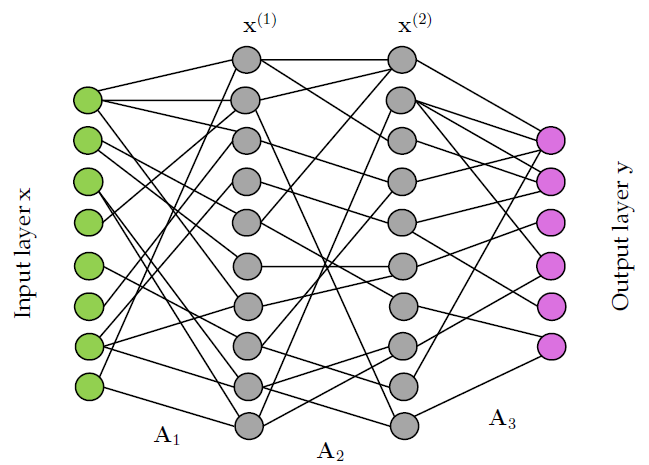
\includegraphics[scale=0.5]{fig/new/RNA.png}
	\caption{Modelo red neuronal artificial. Fuente: \cite{DataScience}.}
	\label{fig:RNA}
\end{figure}

Por lo tanto, la salida de una capa es entonces:

\begin{equation}
\mathbf{x}^{(n+1)} = f(\mathbf{A}, \mathbf{x}^{(n)})
\end{equation}

La red neuronal completa se modela con la composición de $M$ capas de la forma \cite{DataScience}:

\begin{equation}
\mathbf{y} = f_M \left( \mathbf{A}_M ,... , f_2 (\mathbf{A}_2, f_1(\mathbf{A}_1 , \mathbf{x}))  \right)
\end{equation}


La función de activación más utilizada en la actualidad, por el bajo costo computacional que representa, sumado a características teóricas que propician el funcionamiento correcto de los procesos de aprendizaje, es la llamada función ReLU \cite{DataScience}.

\begin{equation}
f_{ReLU}(x) = \left\{ \begin{array}{ll}
0 & \mbox{para $x \leq 0$} \\
x & \mbox{para $x > 0$}
\end{array}
\right.
\end{equation}

En síntesis, estos modelos neuronales tienen capacidad de aproximar cualquier función, ajustando el número de capas, el número de neuronas, y las funciones de activación. El objetivo con estos modelos es, dado un conjunto de entrenamiento con datos de entrada $\mathbf{x}$ para los que se conoce la salida $\mathbf{y}$, y dado un proceso de optimización, ajustar los pesos de cada capa, para que la diferencia entre las salidas que predice el modelo y las salidas $\mathbf{y}$ del conjunto de entrenamiento se minimice poco a poco, hasta que el sistema ``aprenda'' a reproducir esas predicciones, generalizando lo aprendido incluso a patrones de entrada no vistos durante el proceso de entrenamiento \cite{DataScience}.


\section{Aprendizaje reforzado}

En el aprendizaje reforzado (RL por sus siglas en inglés) se parte del supuesto que un agente debe aprender a interactuar en un entorno, de modo que a través de las acciones que el agente ejecuta en ese entorno, se maximice alguna función de recompensa. El agente tendrá algún estado que lo caracteriza (como su posición, su velocidad, etc.) y podrá realizar observaciones sobre el entorno, para decidir qué acciones tomar. Esto se ejemplifica en la figura \ref{fig:esquemaRL} \cite{DataScience}.

\begin{figure}[hh]
	\centering
	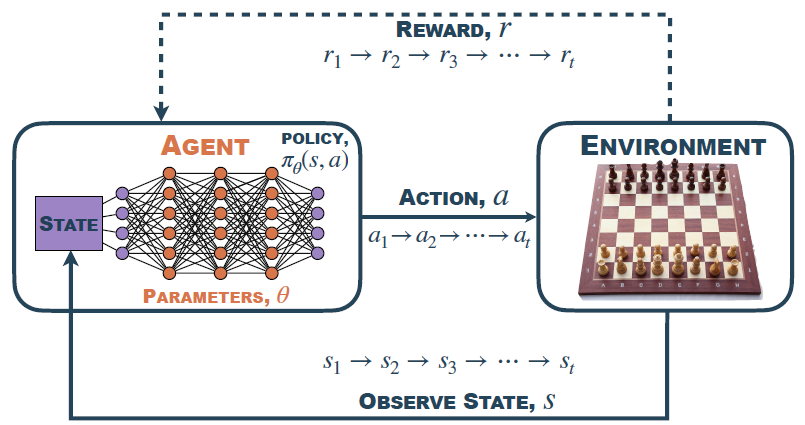
\includegraphics[scale=0.5]{fig/new/ReinforcementLearning.png}
	\caption{Etapas básicas del RL. Fuente: \cite{DataScience}.}
	\label{fig:esquemaRL}
\end{figure}

\subsection{Conceptos base del RL}

\subsubsection{Política}

En aprendizaje reforzado se conoce como política (\textit{policy}) a la estrategia que utiliza un agente para decidir qué acción $a$ tomar, dado su estado actual observable $s$. Existen varias formas de modelar las políticas. Por un lado, en los métodos de aprendizaje reforzado clásicos, la política es una función $\pi$ determinista que mapea de estados a acciones, mientras que métodos más recientes tienden a expresar la política como  \cite{DataScience}:
\begin{equation}
\pi (s,a) = Pr(a=a|\,\, s=s)
\label{ecu:policy}
\end{equation}
donde la política $\pi (s,a)$ es una función que expresa la probabilidad de tomar una acción $a$ dado un estado $s$.


\subsubsection{Recompensa}

La función de recompensa calcula a partir del estado actual del agente, y de la acción a tomar, una magnitud que indica qué tan bién está realizando el agente su tarea. Es la única realimentación que tiene el agente sobre su labor y es la única información disponible para que los algoritmos de aprendizaje reforzado decidan cómo deben mejorar esa recompensa.

Al maximizar las recompensas acumuladas, el agente puede determinar qué acciones son más beneficiosas para alcanzar objetivos a largo plazo. Por lo tanto, el diseño de una función de recompensa adecuada es esencial, ya que moldea el comportamiento del agente e impulsa el proceso de aprendizaje hacia los resultados deseados \cite{RLIntro}.

Una función de recompensa bien definida no solo anima al agente a alcanzar objetivos específicos, sino que también garantiza que el proceso de aprendizaje se mantenga estable y eficiente. Si la señal de recompensa es escasa o está mal definida, el agente tendrá dificultades para identificar patrones significativos a partir de sus interacciones, lo que conduce a comportamientos no deseados \cite{RLIntro}.


\subsubsection{Procesos de decisión de Markov (MDP)}

De manera simplicada, un $MDP$ es un formalismo para modelar un sistema en un estado específico de manera que la probabilidad de pasar a un nuevo estado depende únicamente del estado anterior del sistema y de la acción tomada \cite{DataScience}. 

De manera general, en un $MDP$ la dinámica del sistema se determina con las probabilidades de transición de un estado $s_k$ en el instante $k$ a un estado $s_{k+1}$ en el instante $k+1$ y con la acción $a_k$:
\begin{equation}
P(s', s, a) = Pr(s_{k+1}=s'\,|\, s_k=s, a_k=a)
\end{equation}

Los algoritmos clásicos de RL procuran aprender de la experiencia estas probabilidades y con ellas intentar maximizar la recompensa esperada en una sucesión óptima de estados y acciones. Este proceso es en general complejo, y por ello las técnicas modernas evitan tener que aprender la dinámica del sistema de forma explícita, y buscan formas en que solo implícitamente estas probabilides se aprendan \cite{DataScience}.

\subsubsection{Paso}

Un paso (\textit{step}) en el área de RL define la unidad básica de interacción entre un agente y su entorno. Tomando prestada la terminología de los sistemas de control, un paso se refiere a un único ciclo dentro del bucle de RL, como se muestra en la figura \ref{fig:esquemaRL}. Además, se describe en RL \cite{RLIntro}, el concepto, donde en cada paso, el agente realiza una acción en el entorno, observa el estado resultante y recibe una señal de recompensa, por lo que en un paso ocurre el intercambio de información entre los principales actores del proceso \cite{DataScience}.


\subsubsection{RL con redes neuronales}

Dado que las funciones de probabilidad que representan la dinámica del sistema, las políticas o incluso, en ocasiones, las mismas funciones de recompensa, deben aprenderse a partir de la experiencia del agente interactuando con su entorno, es natural que para estos procesos de aprendizaje se utilicen redes neuronales artificiales (RNA) como modelos de aproximación de esas funciones, aprovechando sus propiedades de aproximadores universales \cite{RLIntro}.

Las técnicas de aprendizaje reforzado que usan redes neuronales proponen entonces estrategias de recolección de los datos con los que se entrenará la red, los valores de referencia o funciones de pérdida que se utilizan para entrenar esas redes, y las estrategias de cómo usar los aprendizajes parciales mientras las redes aprenden en todo el proceso de interacción \cite{RLIntro}.

Como no se conoce lo que debe hacer un agente para mejorar sus espectativas de recompensa, se convierte en un reto plantear los problemas de entrenamiento de las redes neuronales, utilizando únicamente las recompensas o castigos a los comportamientos.


\subsubsection{Etapas de exploración y explotación}

Durante el entrenamiento de un agente por medio de aprendizaje reforzado, se debe asegurar mantener un balance entre las llamadas etapas de exploración y explotación \cite{RLIntro}.

La etapa de exploración incentiva al agente a tomar riesgos y elegir acciones aleatorias, solo para adquirir la experiencia de nuevas posibilidades de obtener mejores recompensas. En la etapa de explotación, el agente usa la política que ha aprendido previamente para determinar qué acciones tomar, con el riesgo de que sea muy conservador y no tome riesgos para aprender nuevas cosas, limitándolo a repetir experiencias que ya conoce \cite{RLIntro}. 

Los algoritmos o métodos de RL usualmente aplican la etapa de exploración al inicio de los entrenamientos de modelos para exponer al agente a situaciones que signifiquen una mayor recompensa. Con el avance del entrenamiento, se utilizan cada vez más las etapas de explotación, de modo que el agente aplica cada vez más las estrategias aprendidas para obtener su recompensa.

Una de las técnicas más utilizadas para lograr el balance entre la exploración y explotación en un entrenamiento se conoce como avaro-$\varepsilon$ (\textit{greedy-$\varepsilon$}). La técnica trabaja con una selección aleatoria, tal que con una probabilidad $\varepsilon$, el agente toma acciones aleatorias y con probabilidad $1-\varepsilon$ toma acciones dadas por la política aprendida \cite{RLIntro}.

El efecto del cambio de $\varepsilon$ se ejempifica en la figura \ref{fig:greedy_eps}, donde se aprecia la afectación de la selección de $\varepsilon$: un $\varepsilon=0$ (curva verde) provoca solo acciones aprendidas que no convergen a una recompensa máxima, mientras que el caso de $\varepsilon = 0.01$ y $\varepsilon = 0.1$ (curvas roja y negra, respectivamente) la exploración en ambas etapas resulta en una mejora progresiva de la recompensa. La velocidad de la convergencia hacia el máximo, varía asociado a qué tanto se le permite al agente explorar \cite{RLIntro}.


\begin{figure}[hh]
	\centering
	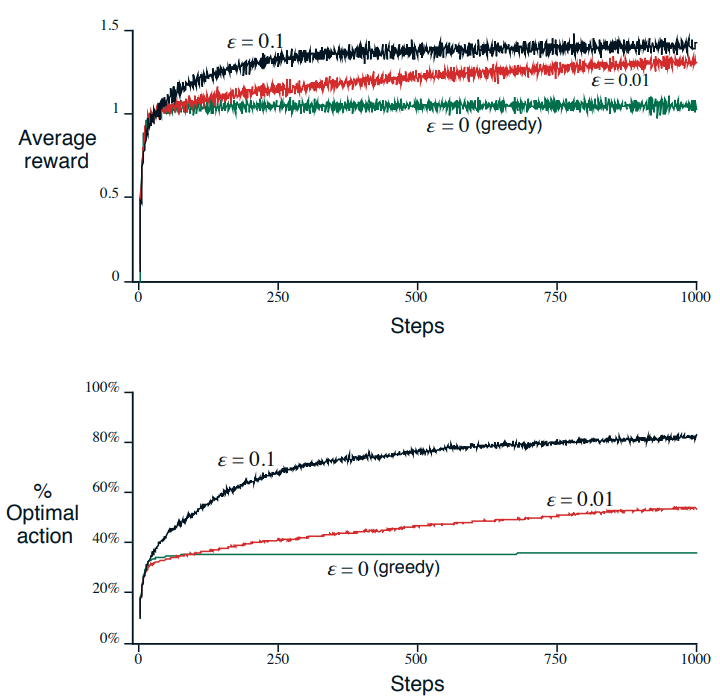
\includegraphics[scale=0.6]{fig/new/avaro_eps.png}
	\caption{Efecto de la selección de la probabilidad $\varepsilon$ en el desempeño del agente. Fuente \cite{RLIntro}.}
	\label{fig:greedy_eps}
\end{figure}


\subsubsection{Categorización del RL}

El RL dirige a los agentes a mejorar la recompensa en función de la política establecida para el control. Dada esa búsqueda del mejor desempeño en los entornos, se han propuesto numerosas técnicas o algoritmos para el RL, lo que se resume en la figura \ref{fig:RLcategorias}. Las categorías principales son: el RL basado en modelos y el libre de modelos. De igual forma se cuenta con el aprendizaje reforzado profundo (DRL), una combinación y reestructuración de métodos de cada subdivisión basada principalmente en las redes neuronales artificiales (RNA) con hasta cientos o miles de capas \cite{DataScience}.

\begin{figure}[hh]
	\centering
	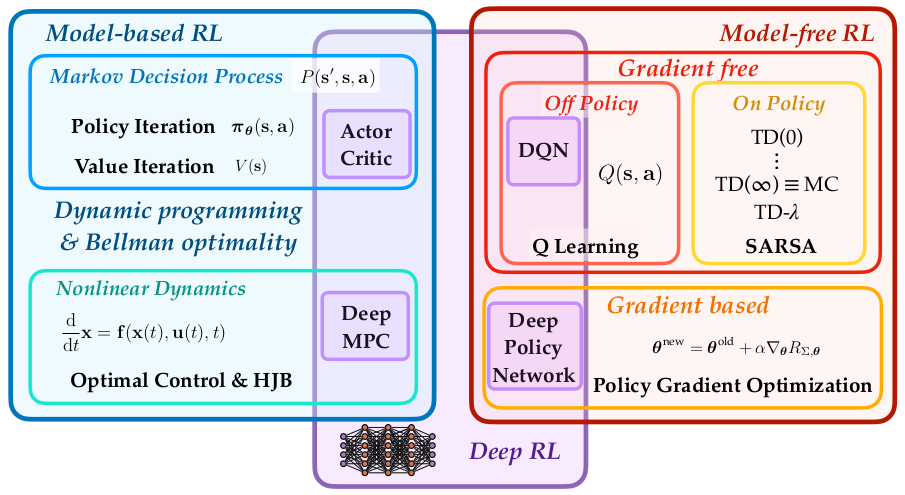
\includegraphics[scale=0.35]{fig/new/CatRL.png}
	\caption{Resumen de categorización del RL \cite{DataScience}.}
	\label{fig:RLcategorias}
\end{figure}

Cada método cuenta con sus premisas que los hacen adecuados para sistemas o entornos particulares, de manera que la identificación de los factores clave del entorno a controlar y su correcta caracterización permiten dirigir la selección de los métodos de RL. En esta ocasión se describen los algoritmos que se seleccionaron como posibles candidatos para el controlador del entorno PAMH.


\subsection{Deep Q-Network (DQN)}

El algoritmo (\textit{Deep Q-Learning}, DQL) es un método de aprendizaje reforzado introducido por la compañía DeepMind Technologies (hoy Google DeepMind) en el año $2013$. El DQL usa RNA para aproximar los llamados valores Q, por lo que se suele definir al método como DQN (\textit{Deep Q-Network}) \cite{DQNbase}. 

Los valores Q provienen del algoritmo clásico de aprendizaje Q (\textit{Q-learning}). Como se observa en la figura \ref{fig:RLcategorias}, se trata de un método fuera de política (\textit{off-policy}), de manera que el aprendizaje de un agente se realiza mediante la exploración de acciones que no siguen la política que haya aprendido el sistema \cite{DataScience}\cite{DQNexplained}. Se define el valor $V(s)$ en un estado $s$ como la recompensa esperada en el estado $s$, si se siguiera una política óptima a partir de allí, o en otras palabras, la mejor recompensa esperable a partir del estado $s$. El valor Q es similar, y se relaciona con el valor $V(s)$ con:
\begin{equation}
V(s) = \max_a Q(s,\,\, a)
\end{equation}

Es decir, el valor Q representa la recompensa total esperada al tomar una acción en un estado dado, siguiendo una política óptima a partir de allí.

\begin{comment}

En esos métodos clásicos se usa programación dinámica para su estimación, pero se requiere conocimiento de la llamada "dinámica del sistema", descrita a través de probabilidades de transición entre estados, dadas las acciones. pero dichas probabilidades suelen ser difíciles de determinar. Por eso aprendizaje Q opta por aproximar la estimación de Q con redes neuronales.

\end{comment}


Aprendizaje Q usa la técnica avaro-$\varepsilon$, de manera que con probabilidad $\varepsilon$ el algoritmo utiliza una acción $a_t$ aleatoria del espacio de acciones (exploración). Caso contrario, con probabilidad $1-\varepsilon$ se toma la acción directa de la respuesta de la RNA (explotación) con:
\begin{equation}
a_t = \arg \max_a Q^*(\phi(s_t), \,\, a;\,\, \theta)
\label{ecu:accionDQN}
\end{equation}
donde $\phi(s_t)$ es un mapeo del estado $s_t$ a un espacio de mayor dimensión y $\theta$ corresponde a los pesos de la estructura de la red neuronal. 

Las acciones y estados tomados se guardan en lotes para la valoración de sus recompensas respecto a la estimación de valores del lote, donde se les calcula una pérdida $L(\theta)$ para evaluar su desempeño con \cite{DQNbase}:
\begin{equation}
target_j = \left\{ \begin{array}{ll}
r_j & \mbox{para estado terminal $\phi_{j+1}$} \\
r_j + \gamma \,\, \max_{a'} Q(\phi_{j+1},\,\, a';\,\, \theta) & \mbox{para el resto $\phi_{j+1}$}
\end{array}
\right.
\end{equation}
\begin{equation}
L(\theta) = E \left[(target_j - Q(\phi_j,  \,\, a_j;\,\, \theta))^2\right]
\end{equation}
donde $target_j$ es la referencia objetivo del lote anterior y el término $Q(\phi_j,  \,\, a_j;\,\, \theta))$ corresponde a la predicción. Desde este punto es necesario aplicar el descenso de gradiente a la función de pérdida y actualizar los valores Q. Una cantidad $N$ de iteraciones aseguran la convergencia del modelo a los valores deseados y por ende, comportamientos deseados del entorno \cite{DataScience}\cite{DQNbase}.

\subsection{Optimización de política próxima (PPO)}

Se trata de un método basado en política (\textit{on-policy}) propuesto en $2017$ por la empresa OpenAI que aprende directamente a predecir la acción para espacios de estado discretos y continuos. Se busca cumplir una política definida y optimizarla poco a poco con actualizaciones. El método nace con la necesidad de utilizar un algoritmo de mayor accesibilidad en su implementación, al contrario de métodos similares pero de mayor complejidad, como el TRPO (\textit{trust region policy optimization}) \cite{PPObase}. 

Entre las funciones clave del método PPO se encuentra la razón de los pesos de la política actual respecto a la anterior, con base en la función de política (\ref{ecu:policy}):
\begin{equation}
r_t (\theta) = \frac{\pi_\theta (a_t | \,\, s_t)}{\pi_\theta (a_{t_{old}} |\,\, s_t)}
\end{equation}
que evidencia el cambio respecto a la política anterior y su valoración por medio de la función de pérdida del aprendizaje:
\begin{equation}
L^{CLIP} (\theta) = \mathbf{E}_t \left[min (r_t (\theta) \,\, \mathbf{A}_t ,\,\, clip(r_t(\theta),\,\, 1-\varepsilon,\,\, 1+\varepsilon) \mathbf{A}_t)\right]
\label{ecu:lossPPO}
\end{equation}
donde $\varepsilon$ es un hiperparámetro del algoritmo que asegura que el cambio a la política anterior no sea muy abrupto para el proceso y el vector $\mathbf{A}_t$ corresponde al estimador de la función de ventaja, obtenido mediante la diferencia \cite{PPObase}:

\begin{equation}
\mathbf{A}_t = Q(s,a) - V(s)
\end{equation}

lo cual genera la recompensa ``extra'' que se puede obtener al tomar las acciones $V(s)$ sobre los valores $Q(s,a)$ \cite{PPOadv}.

En suma, a través de un número $N$ de iteraciones, el modelo pule poco a poco la política que va aprendiendo con cada cálculo de la pérdida (\ref{ecu:lossPPO}) y se actualizan los parámetros $\theta$ de la RNA que convergen durante el proceso para alcanzar la política óptima y maximizan la expectativa de recompensa \cite{DataScience}.

\section{Métricas de evaluación}

\subsection{Función de recompensa}

La función de recompensa sirve de guía a los agentes para decidir que acción tomar. Por consiguiente y de acuerdo con el comportamiento deseado, una función de recompensa engloba el objetivo, las preferencias y las restricciones que presenta la tarea, usualmente adquiriendo la información desde las observaciones al entorno e interpretándolas con base en el comportamiento deseado.

Por lo tanto a la hora de diseñar un sistema de RL, crear una función de recompensa y mantener el monitoreo en la misma, permite interpretar el comportamiento el agente y evaluar su desempeño, como en el ejemplo del caso en la figura \ref{fig:greedy_eps} con la recompensa de cada valor de $\varepsilon$ seleccionado \cite{DataScience}.

\subsection{Pérdida del modelo}

El valor de pérdida (\textit{loss}) en RL, como en el caso de la ecuación (\ref{ecu:lossPPO}), suele obtenerse de los cálculos de los gradientes o procesos de optimización, en donde una pérdida baja en RL no garantiza necesariamente un rendimiento óptimo. Principalmente indica que el agente está aprendiendo y mejorando su política basándose en la estructura de recompensas definida y en el algoritmo elegido \cite{DataScience}.

La principal métrica en RL suele ser la recompensa obtenida por el agente, dado que refleja directamente lo bien que el agente ha aprendido a maximizar sus recompensas, pero la pérdida también desempeña un papel crucial a la hora de guiar el proceso de aprendizaje para la actualización de políticas y funciones de valor.



\subsection{Error de posición angular}

Todo problema que incorpora secciones del control automático es evaluado mediante la respuesta a una entrada conocida a la que se le mide el error de estado estacionario, el tiempo de estabilización, el porcentaje de sobreimpulso, entre otros \cite{Nise}\cite{Ogata}.

Todo el proceso debe responder a una exigencia de punto de operación premeditado, en este caso un porcentaje de error de estado estacionario menor al $10\%$.